\chapter{Zat Padat, Zat Cair, Gas}\label{ch:g3:solids-liquids-gases}

Sebuah batu, segelas susu, \omterm{def:g2:air-around-us:air}{udara} di dalam balon: tiga macam zat yang
berperilaku dengan tiga cara yang sama sekali berbeda. Tahun lalu, air
memperlihatkan ketiga wujudnya kepada kita; tahun ini kita menemukan
bahwa \emph{segala sesuatu} berada dalam salah satu dari ketiga wujud
itu --- dan setiap wujud punya aturan yang ketat.

\section{Tiga keluarga zat}

Semua zat di dunia dapat dipilah menjadi tiga keluarga, yang disebut
tiga \emph{wujud}: padat seperti batu, cair seperti susu, \omterm{def:g3:solids-liquids-gases:gas}{gas} seperti
\omterm{def:g2:air-around-us:air}{udara}. Es, air, dan uap adalah contoh pertama kita: satu zat yang
mengunjungi ketiga keluarga itu. Sekarang mari kita pelajari aturan
tiap keluarga.

\section{Zat padat mempertahankan bentuknya}

\begin{definition}[Zat padat]\label{def:g3:solids-liquids-gases:solid}
Zat yang mempertahankan bentuknya sendiri disebut
\emph{zat padat}\index{zat padat}. Sebuah kunci mempertahankan
lekuknya di sakumu, di dalam laci, atau di dalam air. Kamu dapat
memegang zat padat di antara dua jari, dan memindahkannya tidak
mengubah rupanya. Ada zat padat yang keras (batu), ada yang lembut
(roti), ada yang lentur (karet gelang) --- tetapi kalau dibiarkan,
masing-masing mempertahankan bentuknya.
\end{definition}

\begin{example}[Zat padat yang berbutir]\label{ex:g3:solids-liquids-gases:sand}
Pasir tampak melanggar aturan: dituang dari ember, ia mengambil bentuk
timbunannya, hampir seperti \omterm{def:g3:solids-liquids-gases:liquid}{zat cair}. Tetapi amatilah baik-baik: pasir
adalah kerumunan butiran padat yang mungil, dan \emph{setiap butir}
mempertahankan bentuknya dengan sempurna. Tepung, gula, dan beras
memainkan tipuan yang sama --- kerumunan \omterm{def:g3:solids-liquids-gases:solid}{zat padat} kecil yang mengalir
bersama-sama sementara setiap anggotanya tetap padat.
\end{example}

\section{Zat cair mengalir --- tetapi mempertahankan jumlahnya}

\begin{definition}[Zat cair]\label{def:g3:solids-liquids-gases:liquid}
Zat yang mengalir disebut \emph{zat cair}\index{zat cair}: ia tidak
punya bentuk sendiri dan mengambil bentuk wadah mana pun yang
menampungnya. Tetapi zat cair mempertahankan \emph{jumlahnya}: tuang
segelas penuh susu ke dalam mangkuk dan susunya tetap sebanyak itu ---
tidak lebih dan tidak kurang setetes pun, hanya bentuknya yang baru.
\end{definition}

\begin{omfigure}
\begin{tikzpicture}[scale=0.85]
  \draw[thick] (0,1.7) -- (0.25,0.1) -- (1.75,0.1) -- (2.0,1.7);
  \fill[omDef, opacity=0.3] (0.14,0.8) -- (1.86,0.8) -- (1.79,0.1)
    -- (0.21,0.1) -- cycle;
  \node[below, font=\small] at (1.0,-0.2) {gelas};
  \draw[thick] (4.0,1.1) .. controls (4.1,0.15) .. (5.1,0.1)
    .. controls (6.1,0.15) .. (6.2,1.1);
  \fill[omDef, opacity=0.3] (4.05,0.55) .. controls (4.15,0.18)
    .. (5.1,0.14) .. controls (6.05,0.18) .. (6.15,0.55) -- cycle;
  \node[below, font=\small] at (5.1,-0.2) {mangkuk};
  \draw[thick] (8.2,1.7) -- (8.2,0.1) -- (11.0,0.1) -- (11.0,1.7);
  \fill[omDef, opacity=0.3] (8.2,0.45) rectangle (11.0,0.1);
  \node[below, font=\small] at (9.6,-0.2) {piring};
  \node[above, font=\small] at (5.5,1.9)
    {susu yang sama: bentuk baru tiap kali, jumlah selalu sama};
\end{tikzpicture}

{\small Segelas susu dituang dari wadah ke wadah: bentuknya menurut
kepada wadah, jumlahnya tidak menurut kepada siapa pun.}
\end{omfigure}

\begin{proposition}[Zat cair yang diam selalu mendatar]\label{prop:g3:solids-liquids-gases:level}
Permukaan \omterm{def:g3:solids-liquids-gases:liquid}{zat cair} yang diam selalu rata dan mendatar --- sejajar
dengan lantai. Miringkan botolnya: air di dalamnya tidak ikut miring;
permukaannya tetap mendatar sementara botolnya condong.
\end{proposition}

\begin{omfigure}
\begin{tikzpicture}[scale=0.85]
  \draw[thick] (0.3,-0.9) rectangle (2.1,1.7);
  \fill[omDef, opacity=0.3] (0.3,-0.9) rectangle (2.1,0.5);
  \draw[omDef, very thick] (0.3,0.5) -- (2.1,0.5);
  \node[below, font=\small] at (1.2,-1.25) {tegak};
  \begin{scope}
    \clip[rotate around={-28:(6.2,0.6)}] (5.3,-0.7) rectangle (7.1,1.9);
    \fill[omDef, opacity=0.3] (4.6,-1.1) rectangle (7.8,0.5);
    \draw[omDef, very thick] (4.6,0.5) -- (7.8,0.5);
  \end{scope}
  \begin{scope}[shift={(6.2,0.6)}, rotate=-28]
    \draw[thick] (-0.9,-1.3) rectangle (0.9,1.3);
  \end{scope}
  \node[below, font=\small] at (6.2,-1.25) {dimiringkan: airnya tetap mendatar};
\end{tikzpicture}

{\small Miringkan botolnya sesukamu: permukaan airnya menolak ikut
miring. \omterm{def:g3:solids-liquids-gases:liquid}{Zat cair} yang diam selalu terbaring mendatar.}
\end{omfigure}

\begin{example}[Sifat mendatar yang dipakai]\label{ex:g3:solids-liquids-gases:level}
Tukang bangunan memakai hukum ini setiap hari: \emph{waterpas} mereka
adalah jendela kecil berisi \omterm{def:g3:solids-liquids-gases:liquid}{zat cair} dengan satu gelembung; kalau
gelembungnya duduk di antara kedua tandanya, raknya semendatar \omterm{def:g3:solids-liquids-gases:liquid}{zat
cair} di dalamnya. Dan pada waktu sarapan, perhatikan jus di dalam
karton yang dimiringkan: bagaimanapun kamu memiringkannya, permukaan
di dalamnya tetap rata dan mendatar --- sampai ia menemukan mulut
kartonnya.
\end{example}

\section{Gas mengisi segalanya}

\begin{definition}[Gas]\label{def:g3:solids-liquids-gases:gas}
Sebuah \emph{gas}\index{gas} adalah zat yang menyebar sampai mengisi
\emph{seluruh} ruang yang diberikan kepadanya. \omterm{def:g2:air-around-us:air}{Udara} adalah gas: masukkan ke
dalam botol, ia mengisi botol itu sampai ke setiap sudut; bukalah
botolnya di ruangan yang lebih besar, dan ia menyebar ke seluruh
ruangan itu juga. Gas tidak punya bentuk sendiri maupun tempat diam
sendiri --- berilah ia ruang yang lebih luas, dan ia mengambil
semuanya.
\end{definition}

\begin{example}[Parfum yang bepergian]\label{ex:g3:solids-liquids-gases:perfume}
Seseorang membuka botol parfum di salah satu ujung ruangan. Sesaat
kemudian, hidung di ujung \emph{yang lain} sudah menciumnya. \omterm{def:g3:solids-liquids-gases:gas}{Gas}
parfum itu tidak tinggal sopan di dekat botolnya: begitu dilepaskan,
ia menyebar ke seluruh \omterm{def:g2:air-around-us:air}{udara} di ruangan itu, dari sudut ke sudut ---
persis yang selalu dilakukan keluarga \omterm{def:g3:solids-liquids-gases:gas}{gas}.
\end{example}

\begin{omfigure}
\begin{tikzpicture}[scale=0.85]
  \draw[thick] (0,0) rectangle (11,3.0);
  \draw[thick, fill=omMeth, fill opacity=0.4]
    (0.8,0) rectangle (1.4,0.9);
  \node[below, font=\small] at (1.1,-0.25) {botol parfum, baru dibuka};
  \foreach \x/\y in {1.6/1.2, 2.1/0.6, 2.5/1.7, 3.2/1.0, 3.9/2.2,
      4.6/0.5, 5.3/1.5, 6.1/2.5, 6.9/0.9, 7.7/1.9, 8.5/0.4,
      9.2/2.3, 9.9/1.2, 10.4/2.7, 5.8/0.3, 8.9/1.4} {
    \fill[omThm, opacity=0.7] (\x,\y) circle (2.2pt);
  }
  \node[above, font=\small] at (8.3,3.1)
    {sedikit kemudian: parfum di mana-mana};
\end{tikzpicture}

{\small \omterm{def:g3:solids-liquids-gases:gas}{Gas} yang lepas: dilepaskan di satu sudut, ia menyebar sampai
mengisi seluruh ruangan.}
\end{omfigure}

\begin{omfigure}
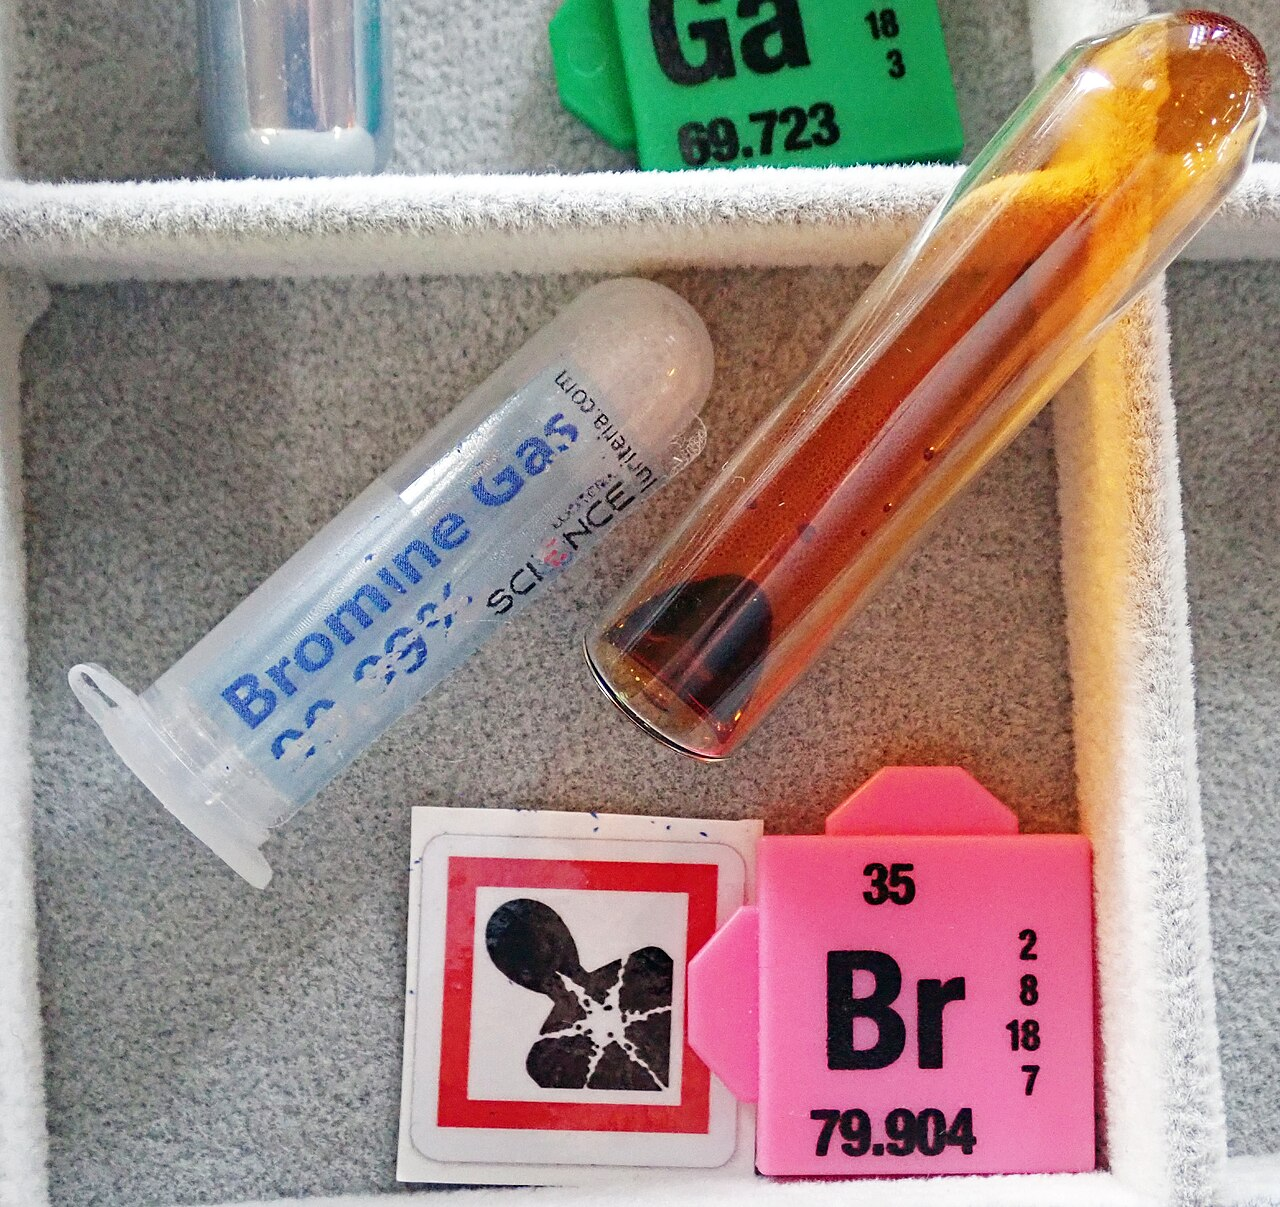
\includegraphics[width=0.4\linewidth, trim={585bp 418bp 15bp 130bp}, clip]
  {images/book1/bromine-gas.jpg}

{\small Kebanyakan \omterm{def:g3:solids-liquids-gases:gas}{gas} tidak terlihat --- tetapi tidak semuanya.
Tabung kaca tertutup ini berisi brom, \omterm{def:g3:solids-liquids-gases:gas}{gas} yang benar-benar berwarna
cokelat jingga: kamu dapat \emph{melihat} \omterm{def:g3:solids-liquids-gases:gas}{gas} itu mengisi setiap sudut
wadahnya, sampai ke kacanya. \emph{Foto: James St.~John, CC\ BY\ 2.0
(dipotong).}}
\end{omfigure}

\begin{remark}[Memilah yang sukar]\label{rem:g3:solids-liquids-gases:tricky}
Ada zat yang perlu diamati dengan cermat. Madu mengalir --- pelan,
tetapi mengalir, mengambil bentuk wadahnya dan mempertahankan
jumlahnya: \omterm{def:g3:solids-liquids-gases:liquid}{zat cair}, hanya saja yang malas. Pasta gigi dan saus tomat
mengalir kalau dipencet: \omterm{def:g3:solids-liquids-gases:liquid}{zat cair} yang kental. Spons adalah \omterm{def:g3:solids-liquids-gases:solid}{zat padat}
yang penuh lubang berisi \omterm{def:g2:air-around-us:air}{udara}. Dan asap? Butiran padat mungil yang
menumpang pada \omterm{def:g3:solids-liquids-gases:gas}{gas} panas. Kalau ragu, ajukan pertanyaan keluarga:
apakah ia mempertahankan bentuknya? apakah ia mengalir? apakah ia
mengisi seluruh ruang yang didapatnya?
\end{remark}

\section{Latihan}

\begin{exercise}[$\star$]\label{exo:g3:solids-liquids-gases:1}
Pilahlah ke dalam tiga keluarga: sekeping koin; \ jus jeruk; \ \omterm{def:g2:air-around-us:air}{udara} di
dalam ban; \ manik-manik kayu; \ minyak; \ \omterm{def:g3:solids-liquids-gases:gas}{gas} uap di atas celah bening
panci yang mendidih.
\end{exercise}

\begin{exercise}[$\star$]\label{exo:g3:solids-liquids-gases:2}
Apa yang dipertahankan \omterm{def:g3:solids-liquids-gases:solid}{zat padat} tetapi tidak dipertahankan \omterm{def:g3:solids-liquids-gases:liquid}{zat cair}?
Apa yang dipertahankan \omterm{def:g3:solids-liquids-gases:liquid}{zat cair} ketika dituang dari gelas ke mangkuk?
\end{exercise}

\begin{exercise}[$\star$]\label{exo:g3:solids-liquids-gases:3}
Sebotol penuh limun dituang ke dalam mangkuk salad yang lebar. Apakah
limunnya sekarang lebih banyak, lebih sedikit, atau sama saja? Apa
yang berubah?
\end{exercise}

\begin{exercise}[$\star$]\label{exo:g3:solids-liquids-gases:4}
Gambarlah akuarium yang terisi air setengahnya: mula-mula berdiri
rata, lalu dimiringkan pada satu tepinya. Gambarlah permukaan airnya
pada keduanya --- ke arah mana permukaan itu terbaring?
\end{exercise}

\begin{exercise}[$\star$]\label{exo:g3:solids-liquids-gases:5}
Bagaimana waterpas tukang bangunan memberitahukan bahwa sebuah rak
sudah mendatar? Hukum mana dalam bab ini yang dipakainya?
\end{exercise}

\begin{exercise}[$\star$]\label{exo:g3:solids-liquids-gases:6}
Mengapa bau panekuk sampai ke kamar tidurmu di lantai atas? Keluarga
mana yang sedang bekerja, dan apa aturannya?
\end{exercise}

\begin{exercise}[$\star$]\label{exo:g3:solids-liquids-gases:7}
Pasir mengucur seperti \omterm{def:g3:solids-liquids-gases:liquid}{zat cair}, namun kita menyebutnya padat.
Jelaskan, dengan \cref{ex:g3:solids-liquids-gases:sand}.
\end{exercise}

\begin{exercise}[$\star$]\label{exo:g3:solids-liquids-gases:8}
Madu memerlukan waktu satu menit penuh untuk mengalir turun dari
sendok. Padat atau cair? Ajukan pertanyaan keluarga pada
\cref{rem:g3:solids-liquids-gases:tricky} lalu jawablah.
\end{exercise}

\begin{exercise}[$\star$]\label{exo:g3:solids-liquids-gases:9}
Keluarga mana yang: mempertahankan bentuknya sendiri? \ mengambil
bentuk wadahnya tetapi mempertahankan jumlahnya? \ mengambil seluruh
ruang yang bisa didapatnya? Sebutkan satu anggota tiap keluarga yang
ada di dapurmu.
\end{exercise}

\begin{exercise}[$\star\star$]\label{exo:g3:solids-liquids-gases:10}
Sebongkah es (padat) \omterm{def:g2:ice-water-steam:meltfreeze}{mencair} menjadi air (cair), lalu matahari musim
panas mengeringkannya menjadi air terbang yang tak terlihat (\omterm{def:g3:solids-liquids-gases:gas}{gas}).
Aturan keluarga mana yang patah pada tiap langkah: apa yang berhenti
dipertahankan zat itu ketika es \omterm{def:g2:ice-water-steam:meltfreeze}{mencair}? ketika air \omterm{def:g2:ice-water-steam:evapcond}{menguap}?
\end{exercise}

\begin{exercise}[$\star\star$]\label{exo:g3:solids-liquids-gases:11}
Sebuah balon ditiup lalu diikat. Mira berkata \omterm{def:g2:air-around-us:air}{udara} di dalamnya
``berbentuk balon, jadi \omterm{def:g3:solids-liquids-gases:gas}{gas} memang punya bentuk''. Jelaskan apa yang
sebenarnya memberikan bentuk itu, dan apa yang akan dilakukan \omterm{def:g2:air-around-us:air}{udaranya}
begitu balon itu meletus.
\end{exercise}
